\subsection{Payment Channel Management}
\label{sec:incentives:channels}

Sending a packet requires the node $n_{open}$ to issue a ticket to the next downstream node $n_{dest}$ which cannot be done without an open payment channel towards $n_{dest}$. So, in order to send a packet, the $n_{open}$ first needs open a payment channel and thereby deposit assets to cover for upcoming tickets that will be issued towards $n_{dest}$.

A payment channel runs throug multiple states during its lifecycle: Initially, each payment channel is \textit{Closed}. Node $n_{open}$ can create one by locking some assets in the smart contract, which leads to \textit{WaitinForCommitment}. This step is necessary because the payment channel becomes usable once $n_{dest}$ has set a commitment. Once that is done, a payment channel is considered \textit{Open}. If the counterparty has already set commitment, then funding immediately changes the state to \textit{Open}. As long as a payment channel is open, the counterparty can submit ticket to redeem them.

Closing a payment channel means accessing the previously locked funds and transfering them to the nodes' accounts. As the smart contract cannot know whether the most recently issued ticket is the last one that got issued and turned out to be a win, payment channels go into \textit{PendingToClose} once $n_{open}$ intends to close it and need to await a timeout once $n_{open}$ is able to retrieve the assets. Before the end of the timeout, the node $n_{dest}$ has the opportunity redeem its stored winning tickets since they lose its validity once the payment channel gets closed. Once the timeout is done, any of the nodes finalize the closure and turn the payment channel state into \textit{Closed}.

\begin{figure}[H]
    \centering
    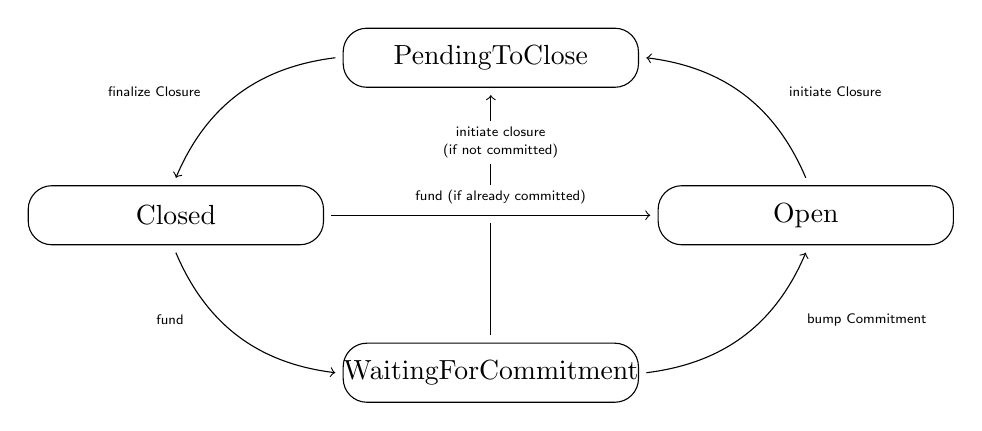
\begin{tikzpicture}[every text node part/.style={align=center}]
        \def\nodeWidth{3.75}
        \def\nodeHeight{0.75}
        \def\padding{0.1}
        \foreach \posX\posY\tag in{0/0/Closed,4/2/PendingToClose,8/0/Open,4/-2/WaitingForCommitment} {
                \draw[rounded corners=3mm,shift={(\posX,\posY)}] (0,0) rectangle (\nodeWidth,\nodeHeight) node[midway] {\smaller{\tag}};
            }

        % Finalize closure
        \draw[->] (4-\padding,2+\nodeHeight/2) to [bend right] (\nodeWidth/2,\nodeHeight+\padding);
        \draw (1.6,1.95) node {\tiny{\textsf{finalize Closure}}};

        % Initiate closure
        \draw[->] (8+\nodeWidth/2,\nodeHeight+\padding) to [bend right] (4+\nodeWidth+\padding,2+\nodeHeight/2);
        \draw (10.25,1.95) node {\tiny{\textsf{initiate Closure}}};

        % Fund
        \draw[->] (\nodeWidth/2,0-\padding) to [bend right] (4-\padding,-2+\nodeHeight/2);
        \draw (1.8,-0.95) node {\tiny{\textsf{fund}}};

        % Bump commitment
        \draw[->] (4+\nodeWidth+\padding,-2+\nodeHeight/2) to [bend right] (8+\nodeWidth/2,0-\padding) ;
        \draw (10.65,-0.95) node {\tiny{\textsf{bump Commitment}}};

        % Initiate closure if not committed
        \draw (4+\nodeWidth/2,-2+\nodeHeight+\padding) -- (4+\nodeWidth/2,\nodeHeight/2-\padding);
        \draw[->] (4+\nodeWidth/2,\nodeHeight/2+\padding) -- (4+\nodeWidth/2,2-\padding);
        \draw (6,1.3) node[fill=white,inner sep=2pt] {\tiny{\textsf{\shortstack{initiate closure\\(if not committed)}}}};

        % Fund if committed
        \draw[->] (\nodeWidth+\padding,\nodeHeight/2) -- (8-\padding,\nodeHeight/2);
        \draw (6,0.6) node[fill=white,inner sep=2pt] {\tiny{\textsf{fund (if already committed)}}};
        % \draw (3,-2.5) node {TODO: add redeemTicket arrows};
    \end{tikzpicture}
    \caption{Payment channel states and possible state transitions.}
\end{figure}

In rare cases it can happen that a node $n_{open}$ intends to open a payment channel, but $n_{dest}$ does not submit an on-chain commitment. Under this circumstance, $n_{open}$ has the opportunity to immediately turn the channel into \textit{PendingToClose}.

\paragraph{State}

Each channel is assigned a unique identifier, computed from the addresses of $n_{open}$ and $n_{dest}$,

$$ channelId = keccak256 (\ ethAddr(n_{open}) \ || \ ethAddr(n_{dest}) \ ) $$

where $ethAddr$ maps public keys to Ethereum addresses. Note that using this scheme leads to different $channelIds$ for the channel from $n_{open} \rightarrow n_{dest}$ and the one from $n_{dest} \rightarrow n_{open}$.

Once $n_{open}$ locks funds, the smart contract instantiates the data structure \textit{ChannelData} and stores it under the previously computed $channelId$ within its storage. Instantiation of \textit{ChannelData} can happen it two ways: either there has been a previous instance of the channel of not. If there has been one, the smart contract keeps the values $commitment$ and $epoch$ from the previous instance. For $epoch$ this is necessary because tickets from previous instances must lose their value once the channel gets closed. This is achieved by incrementing $epoch$ on every incarnation of the channel. On the other hand, commitments are kept to simplify channel reopenings.

\begin{figure}[H]
    \centering
    \begin{tabular}{c|l|c|c|}
        \cline{2-4}
                                                     & \textbf{Value} & \textbf{Ethereum datatype} & \textbf{size (in bytes)} \\
        \cline{2-4}
        \noalign{\smallskip}
        \cline{2-4}
        \multirow{7}{*}{\rotatebox{90}{ChannelData}} & Balance        & uint256                    & 32 bytes                 \\
                                                     & Commitment*    & bytes32                    & 32 bytes                 \\
                                                     & Ticket Epoch   & uint256                    & 32 bytes                 \\
                                                     & Ticket Index   & uint256                    & 32 bytes                 \\
                                                     & Status         & enum                       & 32 bytes                 \\
                                                     & Epoch*         & uint256                    & 1 bytes                  \\
                                                     & Closure Time   & uint32                     & 4 bytes                  \\
        \cline{2-4}
    \end{tabular}
    \caption{The structure of a stored channel. Values marked with * survive reincarnations of the channel.}
    \label{fig:channeldata}
\end{figure}

Closing a channel sets $closureTime$ to current UNIX timestamp plus the timeframe in miliseconds in which node $n_{dest}$ is allowed to submit previously unredeemed tickets. This timeframe is currently set to five minutes for debugging purposes.

\begin{comment}
\paragraph{Opening a channel} Node $A$ can open a channel by transferring funds to the payment channels contract \textit{HoprChannels} and including the following \textit{userdata}:

$$[A: address, B: address, \lambda: uint8, \mu: uint8], \mu = 0,$$

where $\lambda$ is the amount to be staked by $A$. This call will trigger an on-chain event \textit{ChannelFunded} and open a unidirectional payment channel from $A$ to $B$. The payment channel will start in state \textit{Waiting for commitment}. The destination address of the payment channel must now set an on-chain commitment in order for the payment channel between both parties to become \textit{Open}. This is done by $B$ calling the \textit{bumpChannel()} function to make a new set of commitments towards this payment channel. This call will trigger an on-chain event \textit{ChannelOpened} and bumps the ticket epoch to ensure tickets with the previous epochs are invalidated. Every time the channel changes its state, an on-chain event \textit{ChannelUpdated} is emitted.

\paragraph{Redeeming tickets}
As long as the channel remains open, nodes can claim their incentives for forwarding packets via tickets. Tickets are redeemed by dispatching a \textit{redeemTicket()} call to an \textit{Open} payment channel.

If $B$ tries to redeem a ticket from the channel $A\rightarrow B$ (spending channel), but there is an open channel $B\rightarrow A$ (earning channel), $B$'s rewards will be transferred to $B\rightarrow A$ (earning channel). Otherwise, rewards will be sent directly to $B$.

\paragraph{Closing a channel}
Nodes can close a payment channel in order to access their previously staked funds. Only the payment channel creator can initiate the process by calling \textit{initiateChannelClosure()}. This changes the state to $Pending to close$ and triggers a grace period during which the destination node can redeem any unredeemed tickets. Nodes should actively monitor blockchain events to be aware of this payment channel state change.

Once the grace period has elapsed, the payment channel creator can call \textit{finalizeChannelClosure()} which changes the payment channel to $Closed$. When a payment channel is closed, the remaining funds are automatically transferred to the payment channel creator. The channel epoch increments, meaning any unredeemed tickets can no longer be redeemed.
\end{comment}
